\documentclass[11pt]{beamer}

\usetheme{metropolis}

\usepackage{graphicx}
\usepackage{physics}
\usepackage{adjustbox}
\usepackage{caption}
\usepackage{chemformula}
\usepackage{quoting}
\usepackage[style=chem-angew,backend=bibtex]{biblatex}
\bibliography{references}
%
% Choose how your presentation looks.
%
% For more themes, color themes and font themes, see:
% http://deic.uab.es/~iblanes/beamer_gallery/index_by_theme.html
%
\mode<presentation>
{
  \usetheme{default}      % or try Darmstadt, Madrid, Warsaw, ...
  \usecolortheme{default} % or try albatross, beaver, crane, ...
  \usefonttheme{default}  % or try serif, structurebold, ...
  \setbeamertemplate{navigation symbols}{}
  \setbeamertemplate{caption}[numbered]
  \setbeamerfont{footnote}{size=\tiny}
} 

\usepackage[english]{babel}
\usepackage[utf8]{inputenc}
\graphicspath{{../lectureMW/image/}}

\AtBeginSection[]{
\begin{frame}{Outline}
  \tableofcontents[currentsection]
\end{frame}
}

\title{Chapter 7: Electromagnetic Radiation (Light Energy)}
\institute{Chemistry Department, Cypress College}
\date{November 15, 2022}

\begin{document}

\begin{frame}
  \titlepage
\end{frame}

\begin{frame}{Class Announcements}
  \textbf{Lecture}
  \begin{itemize}
  \item Finish Ch 7 and begin Ch 8
  \item Quiz and Homework assignment released Fri, Nov 18th at 3pm
  \item Exam 3 on Nov 22nd; 10 questions covering Exam 2 and
    Chs 7-8
  \end{itemize}
\end{frame}


\section{Review: Periodicity of Electron Configurations}

\begin{frame}{Atomic Orbitals}
  \centering
  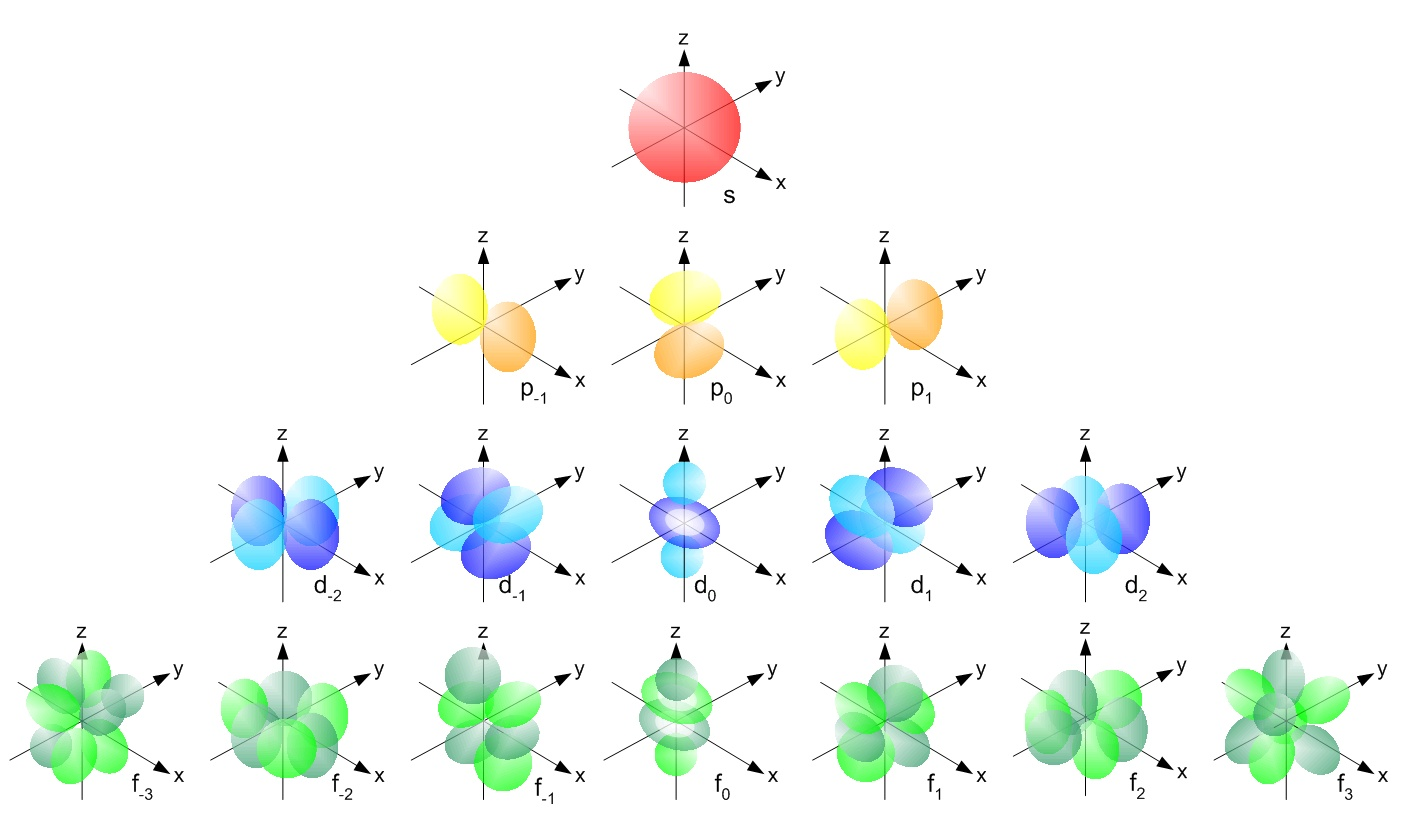
\includegraphics[width=0.8\linewidth]{single_elect_orb}
  \begin{itemize}
  \item Specific orbitals occupy certain \textbf{principal energy level} e.g.
    $n = 1, 2, 3, \cdots$
  \item Basis in which atoms form bond; atomic orbitals combine to make
    molecular orbitals
  \end{itemize}
\end{frame}

\begin{frame}{Orbital Diagram - Multielectron Element}
  \textbf{Q:} What do notice about the relative atomic orbital energies?
  
  \centering
  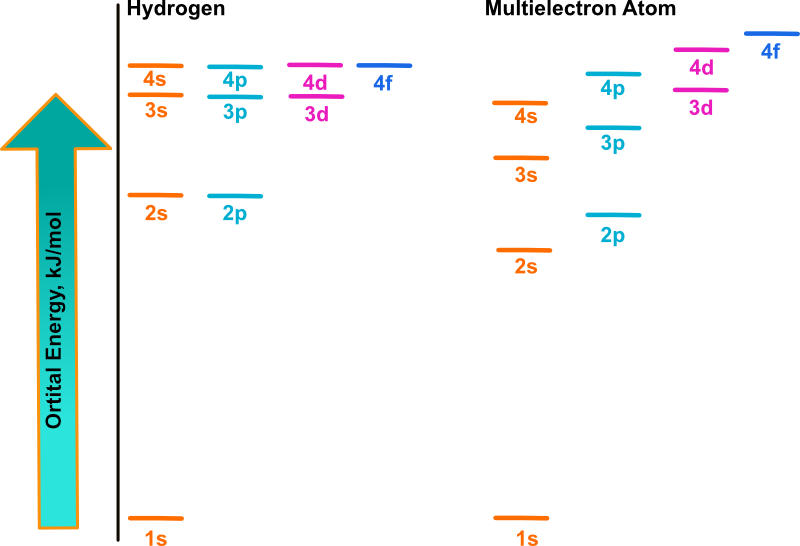
\includegraphics[scale=1.3]{orbital_energy}
\end{frame}

\begin{frame}{Principles for Filling Atomic Orbitals}
  \textbf{Aufbau principle} - electrons fill an orbital starting with
  the lowest energy level

  \textbf{Pauli exclusion princple} - No two electrons with the same
  spin can occupy the same orbital

  \textbf{Hund's Rule} - Maximize the number of unpaired electrons
\end{frame}

\begin{frame}{Relating to Periodic Table}
  \centering
  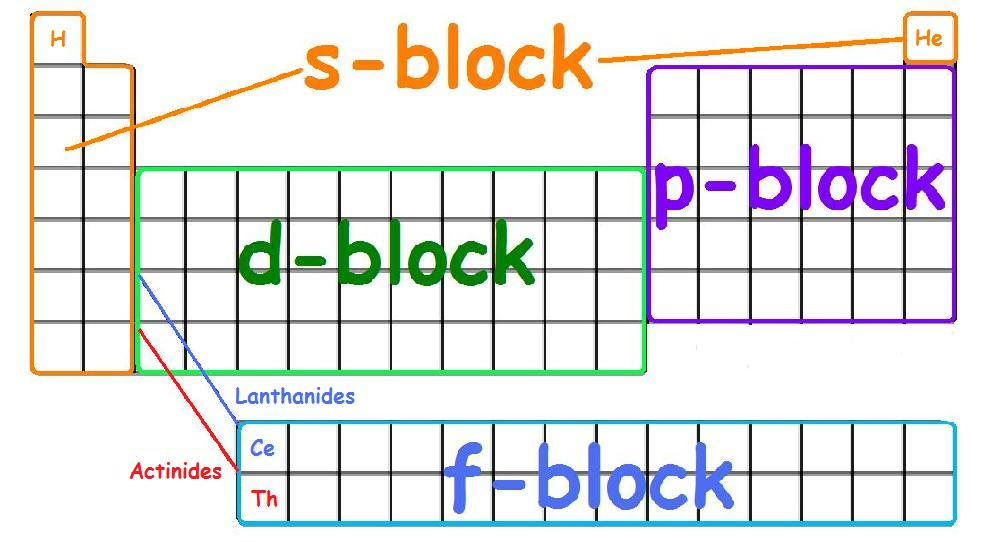
\includegraphics[width=\linewidth]{spdf_orbitals}
\end{frame}

\begin{frame}{Purpose of Electron Configurations}
  \begin{itemize}
  \item Outermost shell is referred to as the valence
    electrons (\textbf{Q:} What is special about valence electrons?)
  \item Innermost shell is the core electrons
  \item Predicts stability of the atom e.g. unfilled orbitals
    indicate instability
  \item Make predictions how elements react forming new chemical
    compounds
  \end{itemize}
\end{frame}

\begin{frame}{Core and Valence Electrons}
  \textbf{Core Electrons} - Energy level $n$ below the valence
  electrons and these are completely filled orbitals

  \textbf{Valence Electrons} - Outermost electrons above the energy
  level $n$ of the core electrons

  \textbf{Example:} Si - $1s^22s^22p^63s^23p^2$
\end{frame}

\begin{frame}{Special Note about d-orbitals}
  Energy levels of 4s and 3d are close along with subsequent $n$ levels
  e.g. 5s and 4d, 6s and 5d
  
  \centering
  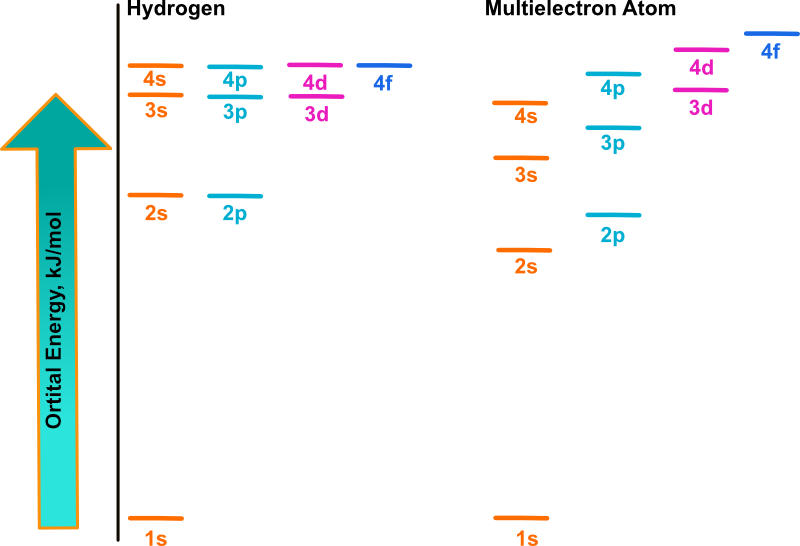
\includegraphics[scale=1.3]{orbital_energy}
\end{frame}

\begin{frame}{Relating to Periodic Table}
  \centering
  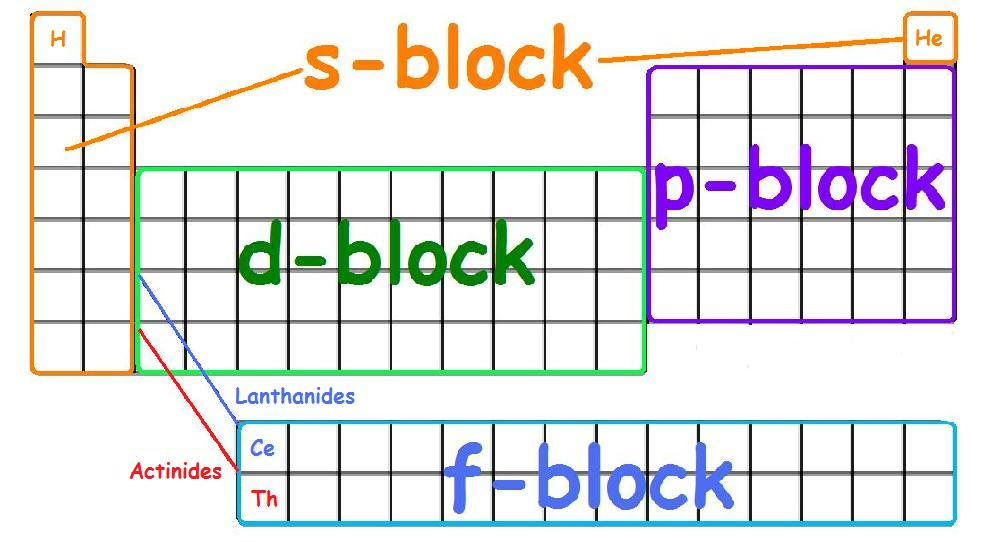
\includegraphics[width=\linewidth]{spdf_orbitals}
\end{frame}

\begin{frame}{Electron Configuration of Ions}
  \textbf{Q:} What is a cation? What is an anion?

  \begin{center}
    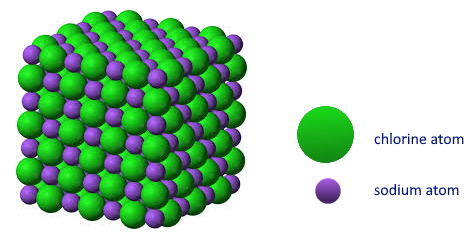
\includegraphics[width=0.7\linewidth]{nacl}
    \end{center}
    
    \textbf{Cation:} Sodium ion (Na$^+$) \textbf{Anion:} Chloride
    ion (Cl$^-$)

  \textbf{Q:} For electron configuration, how do we add/remove
    electrons from atomic orbitals for anion/cation?
\end{frame}

\begin{frame}{Principles for Filling Atomic Orbitals}
  \textbf{Aufbau principle} - electrons fill an orbital starting with
  the lowest energy level
  
  \textbf{Pauli exclusion principle} - No two electrons with the same
  spin can occupy the same orbital

  \textbf{Hund's Rule} - Maximize the number of unpaired electrons
\end{frame}

\begin{frame}{Practice: Writing Electron Configurations}
  \textbf{F$^-$}
  \vspace{0.25in}

  \textbf{Al$^{3+}$}
  \vspace{0.25in}

  \textbf{Na$^+$}
  \vspace{0.25in}

  \textbf{Fe$^{3+}$}
  \vspace{0.25in}

  \textbf{S$^{2-}$}
\end{frame}

\section{Periodic Properties of Atoms}

\begin{frame}{Meaning of Ionization}
  \textbf{Ionization energy} - Energy required to eject an electron
  
  \begin{center}
    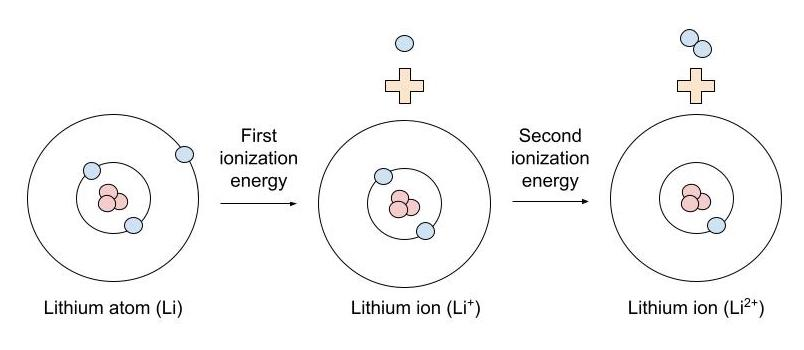
\includegraphics[width=0.8\linewidth]{ionization_Li}
  \end{center}

  First ionization takes 520 kJ/mol and second ionization takes
  7298 kJ/mol

  \onslide<2->{\textbf{Q:} Why is the second ionization energy significantly higher?}
\end{frame}

\begin{frame}{First Ionization Energy Trends}
  \centering
  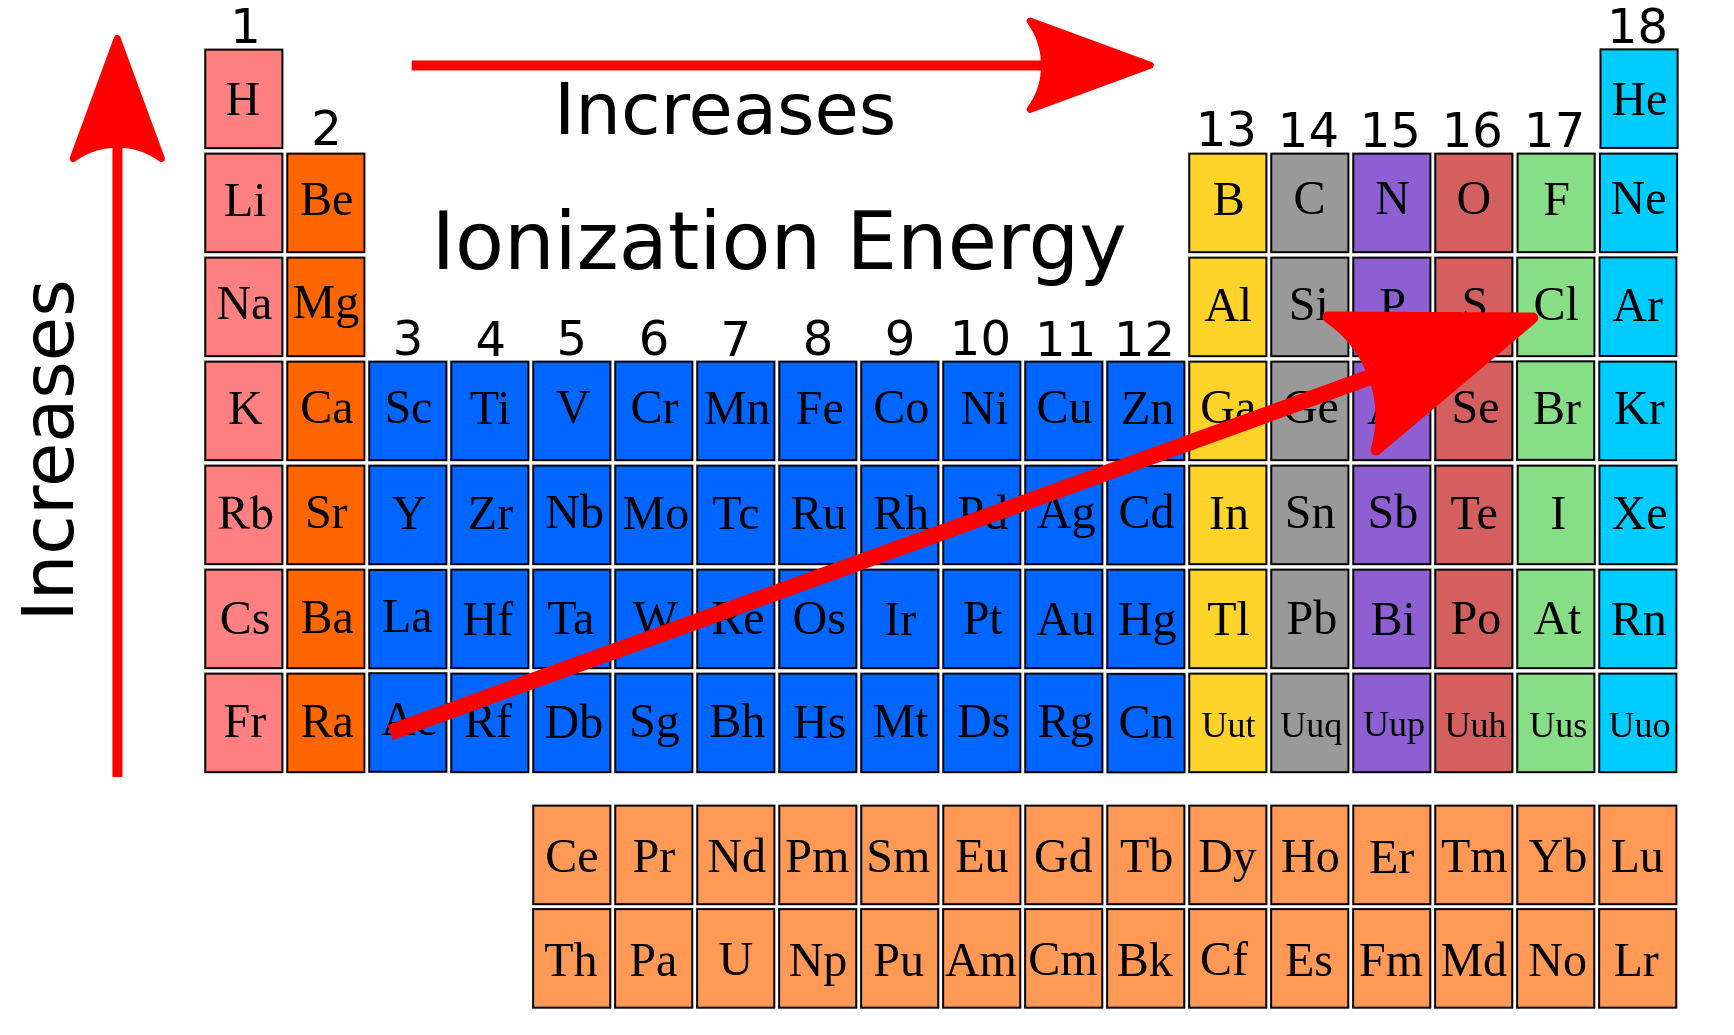
\includegraphics[width=\linewidth]{ion_trends}
\end{frame}

\begin{frame}{First Ionization Energy Trends}
  \centering
  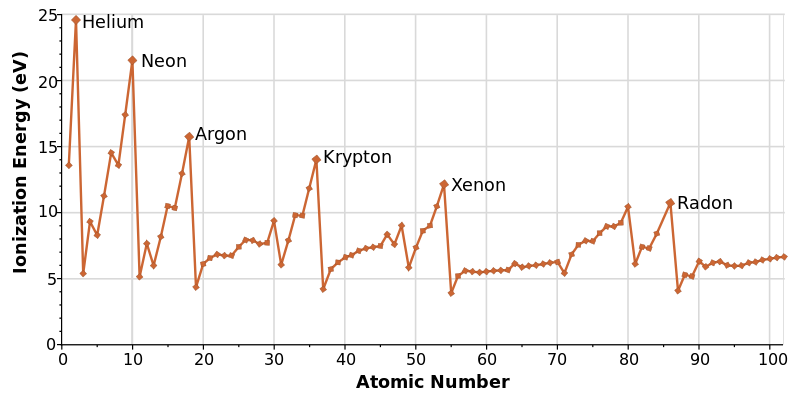
\includegraphics[width=\linewidth]{first-ionization-energy}
\end{frame}

\begin{frame}{Atomic Sizes of Neutral Atoms}
  \centering
  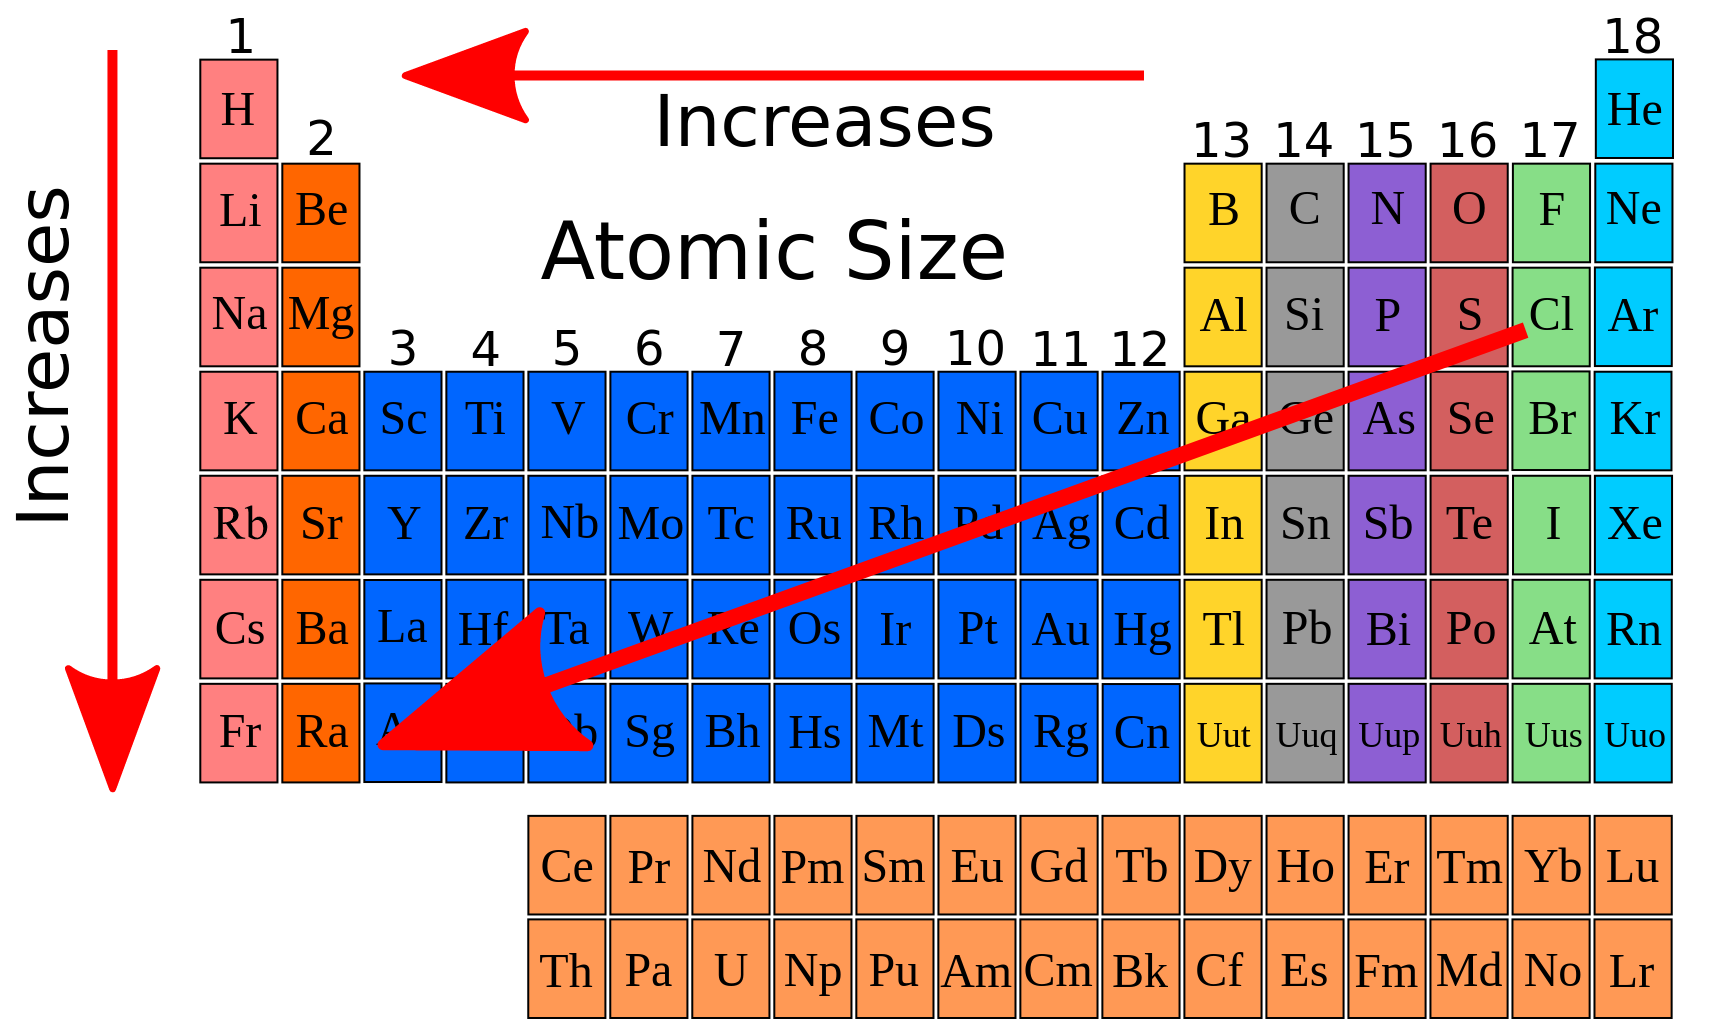
\includegraphics[width=\linewidth]{atomic_trend}
\end{frame}

\begin{frame}{Atomic Sizes of Neutral Atoms}
  \centering
  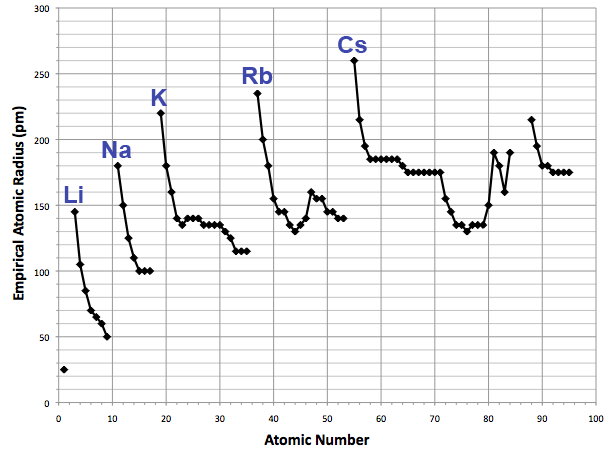
\includegraphics[width=\linewidth]{graph_atomic_rad}
\end{frame}

\begin{frame}{Atomic Sizes of Ions}
  \centering
  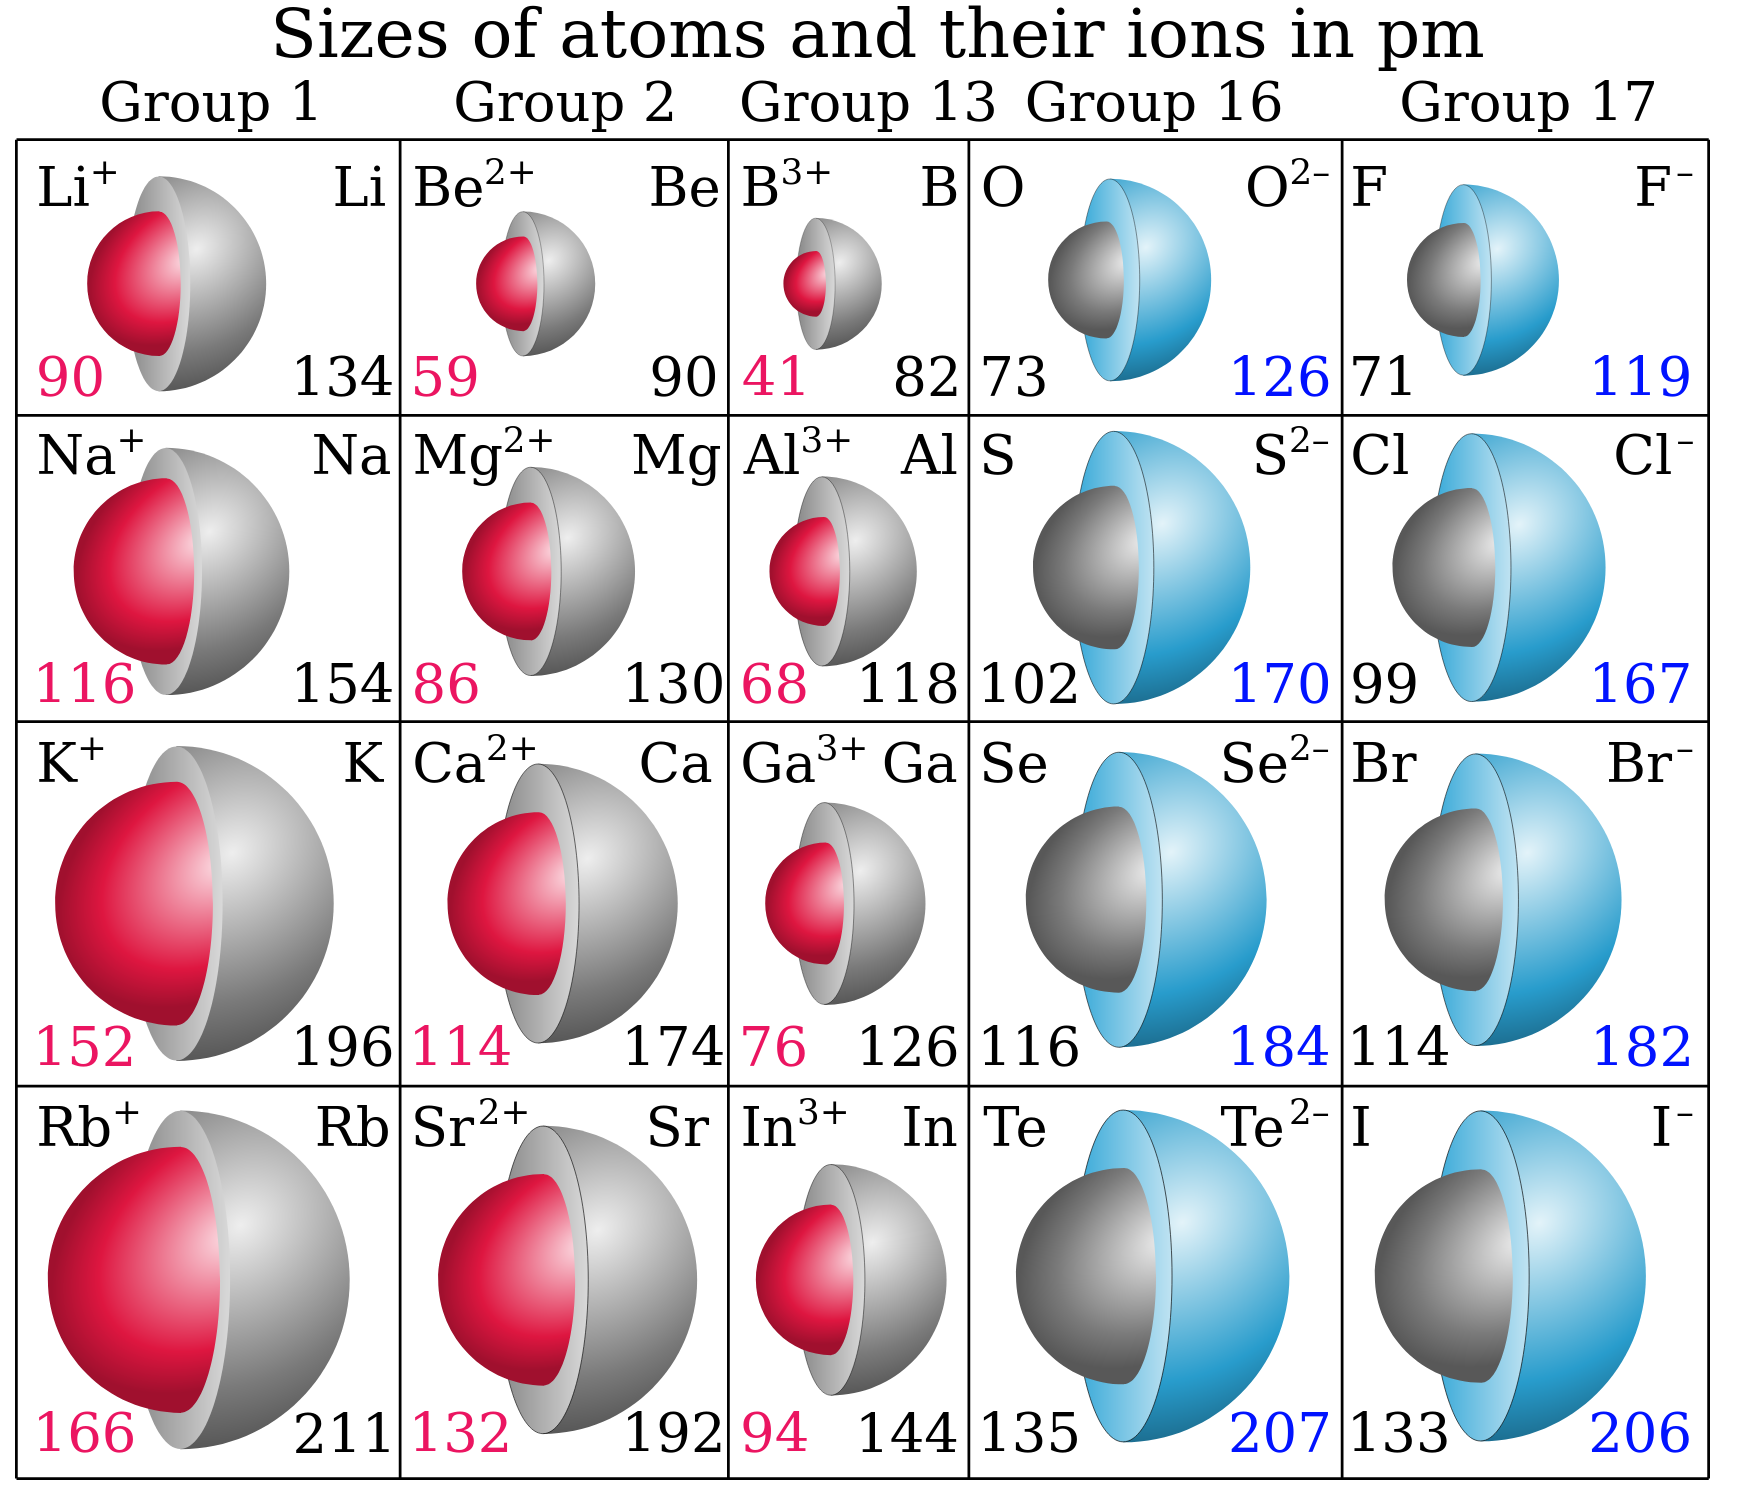
\includegraphics[width=0.8\linewidth]{ion_radii}
\end{frame}

\end{document}
